% This template was created by Ben Mitchell
% for the JHU AI class, CS 335/435, spring 2008. 
% Updated spring 2015 by Ben Mitchell.
%
% Modified by Barbara Holt - Spring 2015
%
% -------------------------------- SETUP:
\documentclass[12pt, letter]{article}
\usepackage[hscale=0.85,vscale=0.85, margin=0.75in]{geometry}

\usepackage{amsmath, amsthm, graphicx}
\usepackage[font={footnotesize}]{caption}
\usepackage[font={footnotesize}]{subcaption}
\usepackage[utf8]{inputenc}
\usepackage[english]{babel}
\usepackage{fancyhdr}
\usepackage{enumitem}
\usepackage{pbox}
\usepackage{float}
\usepackage{morefloats}
\usepackage{wrapfig}
\usepackage{fancyref}

\pagestyle{fancy}
\fancyhf{}
\fancyhead[LE,RO]{B. Holt}
\fancyhead[RE,LO]{Simulating Inquisitiveness and Temporospatial Orientation}
\fancyfoot[CE,CO]{\leftmark}
\fancyfoot[LE,RO]{\thepage}

\renewcommand{\headrulewidth}{2pt}
\renewcommand{\footrulewidth}{1pt}

\setlength{\abovecaptionskip}{0pt}
\setlength{\belowcaptionskip}{0pt}

\def\changemargin#1#2{\list{}{\rightmargin#2\leftmargin#2}\item[]}
\let\endchangemargin=\endlist 

\newlength{\remaining}
\newcommand{\titleline}[1]{%
\setlength{\remaining}{\textwidth-\widthof{\textsc{#1}}}
\noindent\underline{\textsc{\textbf{#1}}\hspace*{\remaining}}\par}

\title{Simulating Inquisitiveness and Temporospatial Orientation With Reinforcement Learning}
\author{Barbara Holt}
\date{May 15, 2015}

\begin{document}
\maketitle

\begin{abstract}
    Reinforcement learning occurs both biologically and artificially through the careful application and manipulation of motivating and constraining variables.  An artificial agent may be trained into various outlooks and perspectives on its environment through stochastic formulas that combine to model real-world learning.  When exploratory functions are applied to reinforcement learning algorithms, agents may become more or less inquisitive about their surrounding environment.  The minimum exploration limit, $N_e$, limits the number of visits to a state-action it takes before a state-action is considered explored.  Data shows that, when varied, $N_e$ may lay across a Bell Curve, with inquisitive behavior varying across it, as well.  Alpha learning functions and the discount factor, gamma, both skew incoming information, orienting an agent's focus further towards or away from future events by limiting their influence on present states.
\end{abstract}

% -------------------------------- INTRODUCTION:
\newpage
\section{Introduction}
Reinforcement learning is an effective tool for training both biological and artificial agents.  Learning occurs through the causal relationship of action and reward or punishment.  Reinforcement refers to the \emph{addition of something} to either encourage or discourage behavior, while punishment refers to the \emph{removal of something} to either encourage or discourage behavior.  For this reason, rewards may also be negative.  

In terms of artificial intelligence, an agent object traverses a carefully controlled environment according to encoded patterns of behavior, or \emph{policies}.  Negative rewards, such as the $-1$ penalty agents incurred in this paper for each iteration an agent was \emph{not} at a terminal state, or finish line position, motivate agents to move toward a particular goal.

This paper focuses on reinforcement learning agents' navigation of the 'Racetrack Problem', a standard control problem where the goal is for an agent, the "racer", to learn to race through a pre-defined track with only the ability to accelerate and decelerate in the x or y direction.  For the following experiments, the world was assumed to be static and all variables discrete for ease of computation.  The velocity in any direction was also capped at 5 to limit the potential state-action permutations.\cite{final}

% -------------------------------- ALGORITHMS & EXPERIMENTAL METHODS:
\section{Algorithms and Experimental Methods}
\titleline{Agents}
Two agents were employed in the battery of experiments described in this paper, the Value-iterating (VI) Agent and the Q-learning (Q) Agent.  Each agent takes a different approach to determining an optimal policy, using state-action pairs, or Q-values, which denote performing a particular action in a certain state or location in an environment.

The Value-iterating Agent approaches the posed scenario by working "backwards" from the goal, and refining a set of values that detail the expected reward of each state-action in the surrounding environment.  In other words, the VI agent assigns and updates a predictive value to each possible state-action, so that upon the subsequent encounter with a particular state-action, the agent might better predict what the most rewarding path is likely to be.

The Q-learning Agent, likewise, assigns values to state-action pairs, but, unlike the VI agent, it updates these values locally as it moves throughout an environment.  This means that value updates do not "spread" to their neighbors, like in VI agent learning, but instead relate only to actions taken and states explored.  In this way, the Q agent's reward prediction suffers until it is has sufficiently explored the entire environment, but it is much more capable of rapid adaptation to new or changing environments.\\

% TRACKS:
\clearpage
\titleline{Tracks}

Seven ASCII Tracks were used during testing and data collection to assess the relative strengths of the learning agents, and the effects of the various learning factors on different problems posed.  All possible starting positions are represented by the letter 'S', while all possible finishing and program-terminating positions are labeled with 'F'.  The agent is randomly placed at a different starting position each iteration.  The agent cannot move to wall positions, denoted by '\#', and movement towards one results in a crash.  However, an element of chance is also introduced, with an agent's intended action only occurring with a $90\%$ likelihood.  In other words, there is a $10\%$ chance that any given action will fail.

\begin{table}[h!]
  \begin{tabular}{c l}
      \raisebox{-1cm}{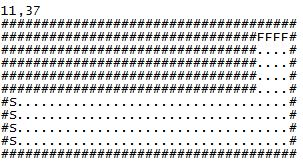
\includegraphics[width=4cm]{img/tracks/L}}
      &
      \pbox{12.5cm}{\textbf{"L" Track} \\ A straight-forward track, the main feature of interest is the open space leading up to the finish-line turn.  This space gives the "race car" agent time to build up velocity, especially if the soft crash setting will allow it to quickly decelerate by "slamming" into walls.  Thus, the L-track is a good test of strategic capabilities for the agent, and we expect to see significant performance changes from hard to soft crash settings.} \\
      
      \raisebox{-2.5cm}{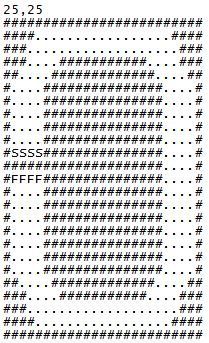
\includegraphics[width=4cm]{img/tracks/O}}
      &
      \pbox{12.5cm}{\textbf{"O" Track} \\ Unlike the L-track, which might reasonably maintain one or two actions for nearly the entire track, this track requires more task-switching and track "experience" to navigate.  With more potential crashes and need to coordinate x and y velocities, we expect to see longer training periods to learn this track.  This is a useful measure for complex task-switching capabilities.} \\
      
      \raisebox{-5cm}{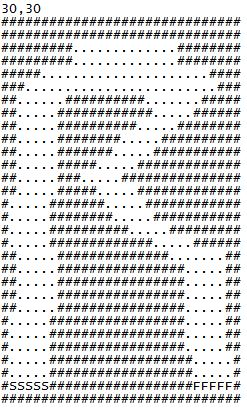
\includegraphics[width=4cm]{img/tracks/R}}
      &
      \pbox{12.5cm}{\textbf{"R" Track} \\ Larger and more complex than the O-track, the R-track alternates between periods of task consistency or persistence (i.e. increasing velocity as the agent traverses the back of the 'R'), and periods of necessary task-switching (i.e. coordinating velocities to turn the head of the R).  The jagged turns at the 'R' tail also invite more crashes if the velocities aren't kept relatively low.  Thus, the 'R' track is a good measure of the interplay between task complexity and the hard versus soft crash settings, the severity of penalty for a difficult track.} \\
      
  \end{tabular}
\end{table}
\clearpage
\begin{table}[h!]
  \begin{tabular}{c l}
      \raisebox{-1cm}{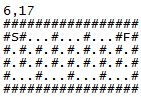
\includegraphics[width=5cm]{img/tracks/Snake}}
      &
      \pbox{11.5cm}{\textbf{"Snake" Track} \\ With only one possible route to take, and an environment that denies velocities of greater than 1 (without crashing), this track focuses on the agent's ability to store complex knowledge, or "memorize" the track.  With only one start and finish position, this also eliminates much of the probabilistic variance of each iteration.  Actions may still misfire, and less "lucky" agents will now be severely penalized.  This allows for a good measure of trial run deviance, and correspondingly, convergence.\\} \\
      
      \raisebox{-2cm}{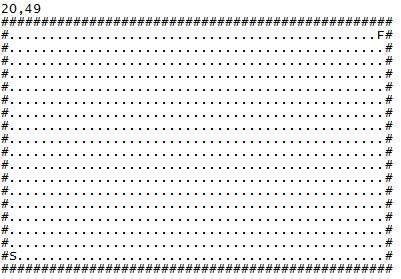
\includegraphics[width=5cm]{img/tracks/Space}}
      &
      \pbox{11.5cm}{\textbf{"Space" Track} \\ The largest track of the seven, Space-track requires more memory space, and more encoded state-action values.  Thus, there is much more room for an agent to get lost, while trying to find the single finish position.  Having again eliminate a randomness factor, this track focuses on, and attempts to control for, an agent's penchant for exploration and its motivation to reach the goal.  We might expect to see the greatest performance changes from exploration function manipulation come from this track.\\} \\
      
      \raisebox{0cm}{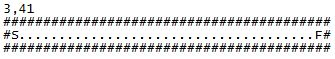
\includegraphics[width=5cm]{img/tracks/Straight}}
      &
      \pbox{11.5cm}{\textbf{"Straight" Track} \\ The Straight-track is a good control for the other tracks, such as the Snake-track.  It even presents the agent with a path of exactly the same length as Snake-track - 39 ground spaces.  Any deficiencies encountered on the Straight-track may be assumed to be agent-based, rather than track-based.  However, this also provides a good measure of task persistence, or the tendency and/or motivation to continue attempting the same task.}
  \end{tabular}
\end{table}

\begin{figure}[h!]
    \centering
    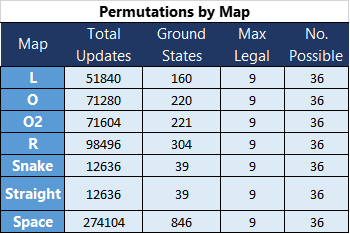
\includegraphics{img/Permutations}
    \caption{Each track requires a different HashMap of values to contain all the possible state-action pairs.  The values for each map are shown here, along with the components used to calculate the total.}
    \label{fig:permutations}
\end{figure}

\newpage

\hfill \break
\titleline{Algorithms}
The two learning agents employed, Value-iterating agent (VI) and Q-learning agent (Q), implement reinforcement learning principles by operating according to the following algorithms:

\begin{enumerate}[rightmargin=.1\linewidth-\leftmargin\relax]
    \item \textbf{Utility Update Equation (\ref{eq:utility})\cite{textbook}}
        Value iteration operates according to the \emph{utility update equation} (\ref{eq:utility}).  Every state-action pair that the agent encounters on a map has a corresponding utility value, the ultimate expected outcome for the agent should it choose to take this particular state-action path.  Whenever a state-action is executed, this value is updated according to the \Fref{eq:utility} below:
        \\
        \begin{equation} \label{eq:utility}
            U^+(s)\leftarrow R(s)+\gamma \cdot max_a f(\sum_{s'} P(s'|s,a)U^+(s'), N_{sa}[s,a])
        \end{equation}
        \begin{small} \begin{changemargin}{1cm}{1cm}
        where $N_{sa}$ is a table of state visitation events, $s$ is the current state, $a$ the current action, $R(s)$ the state's reward, function $P$ the probability of each possible outcome of a state-action, and function $f$ the exploration function (\ref{eq:exploration}).
        \end{changemargin} \end{small}
        
        The update value is calculated by summing together products of all possible outcomes of a state-action and their corresponding probabilities.  In other words, the VI takes a weighted average of the outcome of a particular state-action, $(s,a)$, in an attempt to predict what reward will \emph{most likely} be yielded.  It then compares these weighted averages across all the state-actions it might execute, and selects the maximal option.  The resulting value is fed into the exploration function (\ref{eq:exploration}), along with the number of times this state-action has been "visited", or executed.  The reward returned is then multiplied by the discount factor, or $\gamma$, whose effect is described in the variables section, and added to the reward given by the current state, $s$.  For the purposes of this paper, $R(s)$ will always return $-1$ in non-terminating states, or states other than the finish line positions denoted by 'F'.
        
    \item \textbf{Exploration Function (\ref{eq:exploration})\cite{textbook}}\\
        The \emph{exploration function}, $f$, may take many forms in practice, but is implemented here in a simplistic form:
        \\
        \begin{equation} \label{eq:exploration}
            f(u(s,a),n)=\left\{\begin{matrix}
            R^+ & if n < N_e\\ 
            u(s,a) & if n \geq N_e\\
            \end{matrix}\right.
        \end{equation}
        \begin{small} \begin{changemargin}{1cm}{1cm}
        where $n$ is the number of visitation events of a state-action pair, and $N_e$ is the minimum number of times a state-action should be explored.
        \end{changemargin} \end{small}
        
        This equation is employed in both the VI agent's utility function, and the Q agent's update function to encourage the agent to strike an appropriate balance between exploration and persistence.  A grid of values, $N_{sa}$, keeps track of the number of times each state-action has been executed, or "visited".  The visitation value, or number of times an agent has explored a given state, is denoted by '$n$'.  A constant, $N_e$, acts as an exploration limit.  If a state-action has been visited $N_e$ times or greater, the expected reward is simply the value $u(s,a)$, the reward predicted by the utility function.  Otherwise, the state-action is deemed unexplored or insufficiently explored, and given an optimistic estimate of the possible rewards.  In other words, once a state-action has been visited enough, the agent becomes more "comfortable" with the accuracy of its prediction, while unexplored areas are assumed to be worth looking into or learning about.
    
    \item \textbf{Q-learning Update Equation (\ref{eq:qlearnupdate}), Citation \cite{textbook}}\\
    \begin{equation} \label{eq:qlearnupdate}
        Q\left [ s,a \right ]\leftarrow Q\left ( s,a \right )+\alpha (N_{sa}[s,a])(R(s)+\gamma \cdot max_a' Q\left [ s',a' \right ]-Q\left [ s,a \right ]))
        \end{equation}
        \begin{small} \begin{changemargin}{1cm}{1cm}
        where  $N_{sa}$ is a table of state visitation events, $s$ is the current state, $a$ the current action, $R(s)$ the state's reward, $Q$ the table of state-action values, and $max_a' Q\left [ s',a' \right ]$ represents the maximized expected state-action value from all possible subsequent states $s'$.
        \end{changemargin} \end{small}
        
    Unlike the VI utility update function (\ref{eq:utility}), the Q-learning update equation does not take into account probabilities of all possible outcomes, but adapts to situations as it encounters them.  Algorithmically, this amounts to only looking at the most rewarding possible \emph{next} action, or $max_a' Q\left [ s',a' \right ]$.  The difference between this reward and the value of the current state-action, $Q\left [ s,a \right ]$, is added to the reward of the state, $R(s)$ ($-1$ in this paper), and eventually added back onto the original value, $Q\left [ s,a \right ]$.  By taking the difference between these two values first, the amount of influence for each update may be controlled by the learning factor equation, $\alpha (n)$, and $\gamma$, which will both be discussed in the subsequent sub-section.  Effectively, the expected value of each state-action pair "trickles down" to the state-action pairs behind it, or neighboring it.  This is analogous to the utility function's value dispersal, except that it acts \emph{locally}, rather than \emph{globally} across the entire map each iteration.
    
\end{enumerate}

\titleline{Factors}
\begin{itemize}
    \item \textbf{Alpha Learning Factor/Function}\\ The \emph{alpha learning factor, $\alpha$} determines \emph{the rate} at which an agent learns.  In Eqs. (\ref{eq:utility}) and (\ref{eq:qlearnupdate}), this translates to \emph{how large updates may be}.  For example, in the Q-learning function (\ref{eq:qlearnupdate}), larger values of $\alpha$ will allow greater updates to occur each iteration, while smaller values of $\alpha$ will only allow a partial update, and, thus, require more update events to significantly change the stored value.  Thus, alpha controls how much an agent allows each state-action instance to contribute to learning and influence the overall score.\\
    \\
    When an exploration function (\ref{eq:exploration}) is involved, the alpha learning factor becomes a function of $n$, the number of visitation events discussed in Eq. (\ref{eq:exploration})'s description.  One of the experiments described in this paper considers the effects of different polynomial alpha learning factor functions.
    \item \textbf{Gamma Discount Factor} \\ The \emph{discount factor}, $\gamma$, describes \emph{how much weight an agent places on future events}.  In other words, the discount factor "discounts" events that the agent considers to be \emph{too far into the future} to be considered relevant.  This is why in Eqs. (\ref{eq:utility}) and (\ref{eq:qlearnupdate}) $\gamma$ is multiplied by the $s'$ state reward or utility.  Lower discount factors correspond to lessened \emph{weight} placed on values several steps ahead.  Gamma is also correlated with the rate at which an agent converges on a fixed point, or near-stationary set of state-action values.  More "short-sighted" agents will reach this equilibrium faster than those still weighing equally state-action values several steps ahead.
\end{itemize}

\clearpage
\titleline{Experiments}
\begin{itemize}
    \item \textbf{Experiment 1: Inquisitiveness \& The Necessity for Adaptive Fluctuations - \\The Exploration Function, Crash Penalties, \& Standard Deviation}\\
    One of the most asked machine learning questions comes in the form of the nature of risk and reward.  Here we explore the nature of learning "inquisitiveness" through the manipulation of the exploration function (\ref{eq:exploration}) parameter $N_e$, or the minimum visits limit.  Correspondingly, we view the effects of penalties on inquisitiveness by recording the performance of agents when heavily-penalized through "hard crashes" versus "soft crashes".  Hard crashes send the agent back to the starting line, while soft crashes merely set the agent's velocity to zero, leaving them motionless, but in the same location.  The hard crash setting discourages inquisitiveness, while the exploration function encourages it.  The interaction between the two effects reveals the essential nature of inquisitiveness to learning.\\
    \\
    This experiment also exploits the Q agent's adaptive "learn-as-I-go" nature, comparing its response across various environments.  Each map presents unique challenges, as described in the \textbf{Maps} sub-section.  By exploring the Q agent's resistance to convergence in each situation, we might extrapolate, which tasks require more "thinking" or "learning" by the agent, as well as identify potential weaknesses in the overall Q-learning algorithm.
    \\
    Both the VI and Q agents were tested on all tracks with both the hard and soft crash settings, using a minimum explorations limit, $N_e$, of 1, 2, 4, and 8.  After training the convergence rates were recorded, along with the average performance score and variability across 10 testing simulations.
    
    \item \textbf{Experiment 2: Artificial Time - Convergence Rates by Alpha \& Gamma Factors} \\
    As discussed in the 'Factors' sub-section, an $\alpha$ learning factor function may affect the size of state-action value updates with respect to the number of times a given state-action has been visited, $n$.  An inverse relationship between update weights and the number of visits, this effectively creates a variable update function akin to the discount factor's effect.  Both functions temporally determine update values.  While the alpha factor function is not strictly "time-dependent", the number of visitations events is nonetheless akin to an artificial passage of time.  Thus, comparisons of the effects of the alpha learning function and gamma discount factor speak to the nature and effect of artificial time in machine learning.
    \\
    The Q agent's change in average performance and variability, as well as convergence rate was recorded, while varying, first, the alpha learning factor function, and, second, the values of discount factor $\gamma$.  Results for each were compared and plotted, as presented in the following section.
    \\
    The alpha learning functions used in the assessment included the following variations:
    \begin{equation} \label{eq:alphaN}
        \alpha(n) = \alpha
    \end{equation}
    \begin{equation} \label{eq:alpha10N}
        \alpha(n) = \alpha /(10\cdot n)
    \end{equation}
    \begin{equation} \label{eq:alphaNN}
        \alpha(n) = \alpha /(n\cdot n)
    \end{equation}
\end{itemize}

% -------------------------------- RESULTS:
\clearpage
\section{Results}
\titleline{Experiment 1}

Data collection for Experiment 1 involved the creation of various Q and VI learning agents with varied soft and hard crash settings, as well as minimum explorations values, $N_e$ of 1, 2, 4, and 8.  The Q agent experienced memory heap problems with larger or more complex maps, so under hard crash settings only L-track was tested.  The L-track, O-track, and Space-track were chosen for the Q learner soft crash tests, as they displayed interesting features for an inquisitiveness study (as described in the the 'Maps' sub-section).

Metrics measurements consisted of recording the number of iterations and milliseconds taken for each agent to converge upon an optimal policy, meaning the time taken for a near-equilibrium of stored state-action values to be reached, as well as the final score of each "racer" at the end of ten separate simulations.  The program scored agents by subtracting one point for each iteration the agent spent in a ground state, rather than a terminal finish-line state.  For the Q learner, the 10 trial scores were averaged both before and after convergence.  This allowed the \emph{differences} in both score and the standard deviation of each set of 10 trials to be measured.  Thus, the Q learner results shown below demonstrate the relative change in variation and performance among agents under each set of conditions.

% SOFT VS. HARD Q:
\begin{figure}[h] 
    \centering
    \begin{subfigure}[b]{0.48\textwidth}
        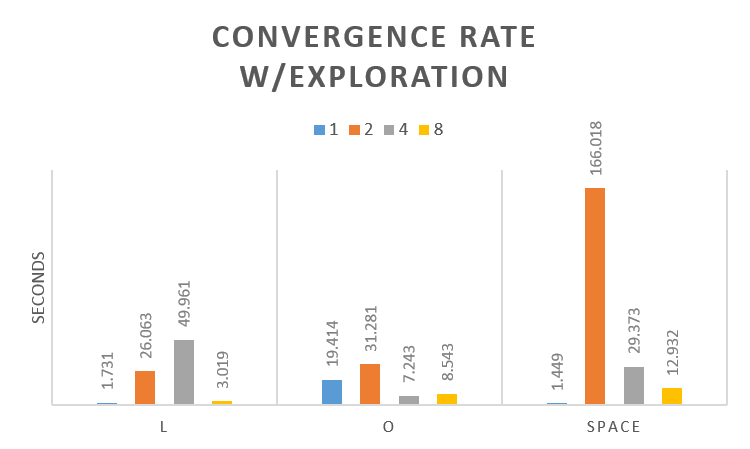
\includegraphics[width=1\textwidth]{img/minE/Time}
    \end{subfigure}
    \begin{subfigure}[b]{0.48\textwidth}
        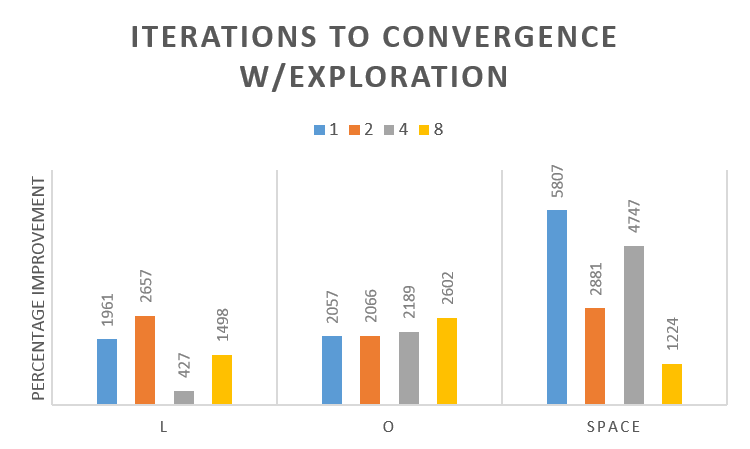
\includegraphics[width=1\textwidth]{img/minE/Iter}
    \end{subfigure}
    \caption{The seconds and iterations taken for a Q agent's state-action values to reach an equilibrium state, or convergence, on maps L, O, and Space are shown above. The minimum exploration value was varied between 1, 2, 4, and 8 under soft crash settings.}
    \label{fig:minETimeIter}
\end{figure}

\begin{figure}[h] 
    \centering
    \begin{subfigure}[b]{0.48\textwidth}
        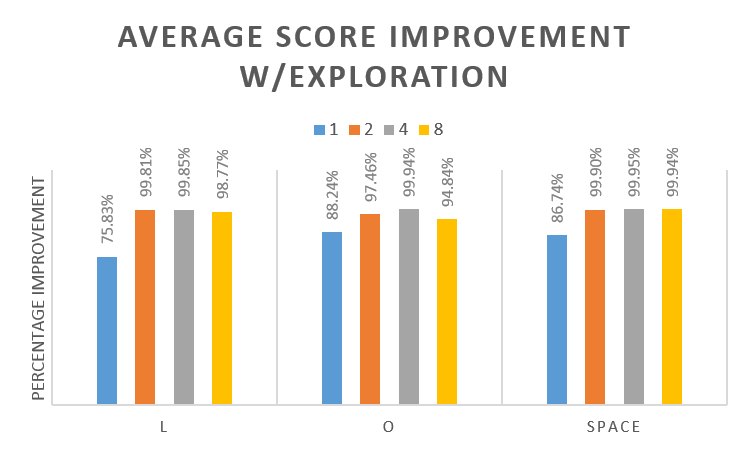
\includegraphics[width=1\textwidth]{img/minE/AvgScore}
    \end{subfigure}
    \begin{subfigure}[b]{0.48\textwidth}
        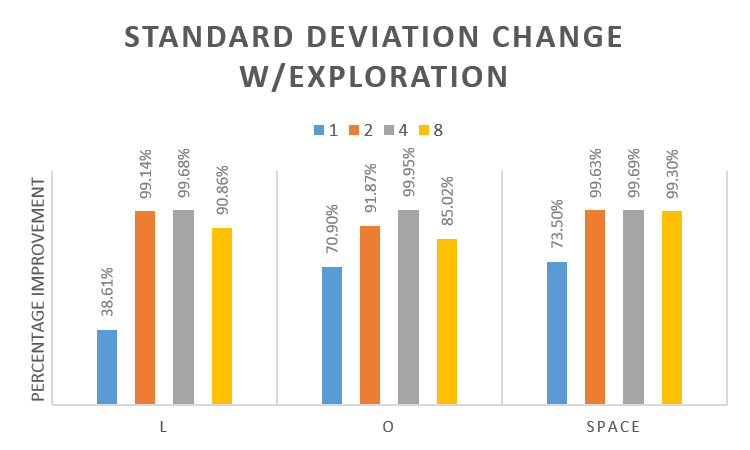
\includegraphics[width=1\textwidth]{img/minE/StDev}
    \end{subfigure}
    \caption{The minimum exploration value for a Q agent was varied between 1, 2, 4, and 8 under soft crash settings.  Simulation score averages were taken across three different maps. Standard deviation analysis measured the variability of scores across the simulations. The results are shown above for each condition.}
    \label{fig:minEAvgScoreStDev}
\end{figure}
\clearpage

After measuring racer performance for different minimum exploration values under \emph{soft} crash settings, agents were subjected to the same array of conditions, but with a hard crash penalty introduced.

\begin{figure}[h] 
    \centering
    \begin{subfigure}[b]{0.49\textwidth}
        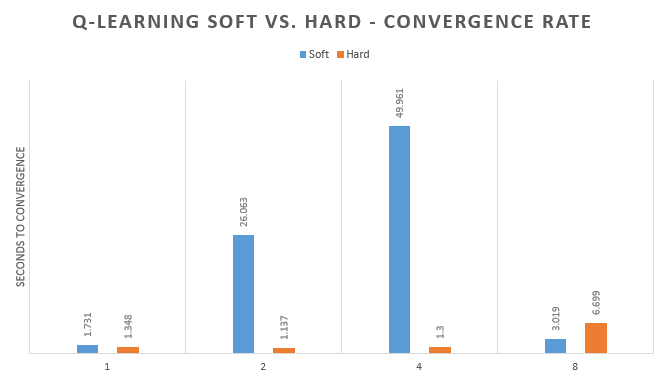
\includegraphics[width=1\textwidth]{img/softVhard/Q/Time}
    \end{subfigure}
    \begin{subfigure}[b]{0.49\textwidth}
        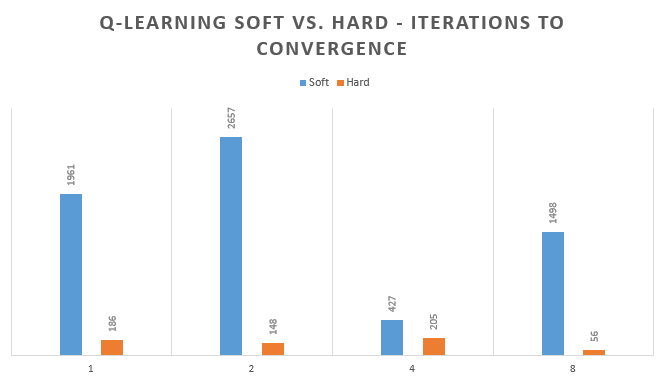
\includegraphics[width=1\textwidth]{img/softVhard/Q/Iter}
    \end{subfigure}
    \caption{Simulated using the L-track, the minimum exploration value for a Q agent was varied between 1, 2, 4, and 8. The seconds and iterations taken for a Q agent's state-action values to reach an equilibrium state, or convergence, are shown above comparing the results from the hard and soft crash conditions.}
    \label{fig:svhQTimeIter}
\end{figure}

\begin{figure}[h] 
    \centering
    \begin{subfigure}[b]{0.48\textwidth}
        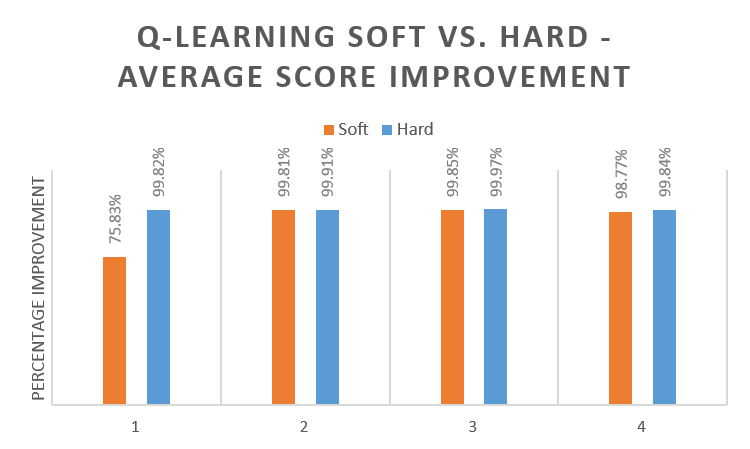
\includegraphics[width=0.9\textwidth]{img/softVhard/Q/AvgScore}
    \end{subfigure}
    \begin{subfigure}[b]{0.48\textwidth}
        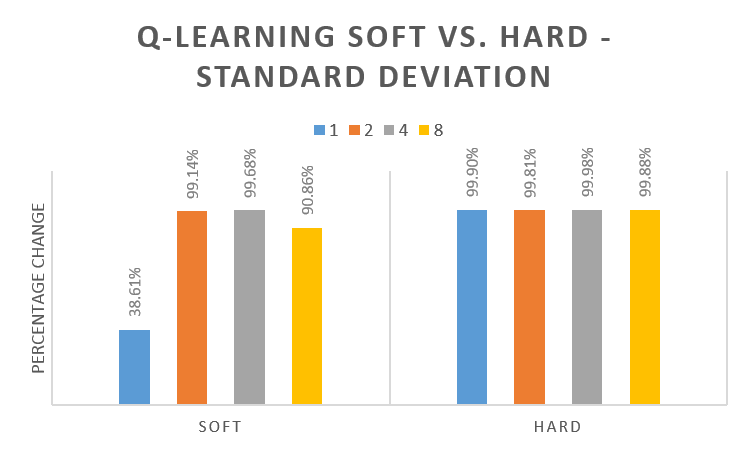
\includegraphics[width=0.9\textwidth]{img/softVhard/Q/StDev}
    \end{subfigure}
    \caption{Simulated using the L-track, the minimum exploration value for a Q agent was varied between 1, 2, 4, and 8. Simulation score averages were taken and standard deviation analysis measured the variability of scores across the simulations. The results are shown above comparing the results from the hard and soft crash conditions.}
    \label{fig:svhQAvgScoreStDev}
\end{figure}

% SOFT VS. HARD VI:
The comparable VI learner results were visited next.  Again, the separate soft crash results are shown first.  These results provide a baseline from which we may view the soft versus hard crash settings comparisons.  Unlike the Q agent results, average scores are presented, rather than the \emph{differences} between average scores, as the VI agent is unable to effectively navigate test maps without adequate training.  Thus, without a measurement of the VI learner's performance \emph{before} convergence, the relative changes are impossible to measure.  Instead, the flat average scores are shown, as evidenced by the negative-value bar graph below.  Since only local map comparisons were informative in this case, all maps were surveyed.

\begin{figure}[h] 
    \centering
    \begin{subfigure}[b]{0.48\textwidth}
        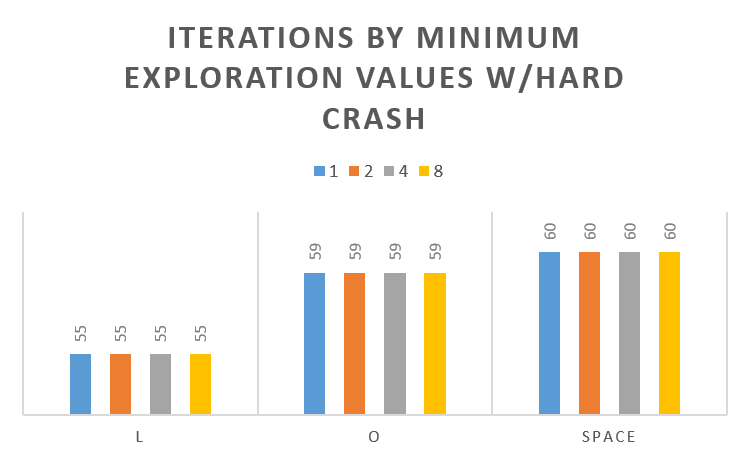
\includegraphics[width=1\textwidth]{img/hard_Iter}
    \end{subfigure}
    \begin{subfigure}[b]{0.48\textwidth}
        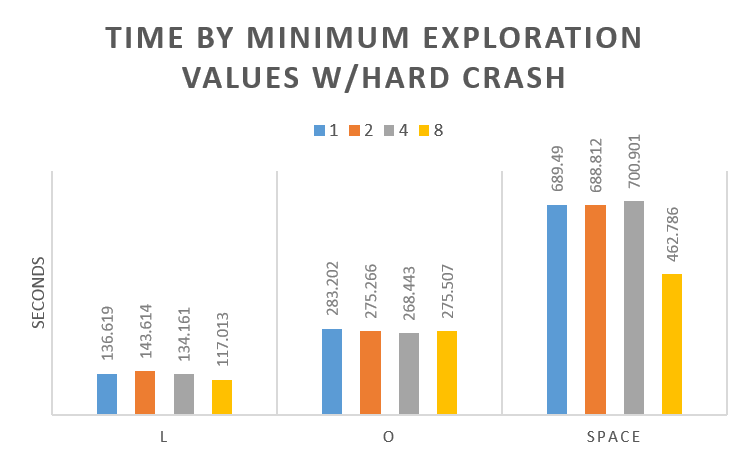
\includegraphics[width=1\textwidth]{img/hard_Time}
    \end{subfigure}
    \caption{The seconds and iterations taken for a Q agent's state-action values to reach an equilibrium state, or convergence, on maps L, O, and Space are shown above. The minimum exploration value was varied between 1, 2, 4, and 8 under hard crash settings.}
    \label{fig:hardTimeIter}
\end{figure}

\begin{figure}[h] 
    \centering
    \begin{subfigure}[b]{0.48\textwidth}
        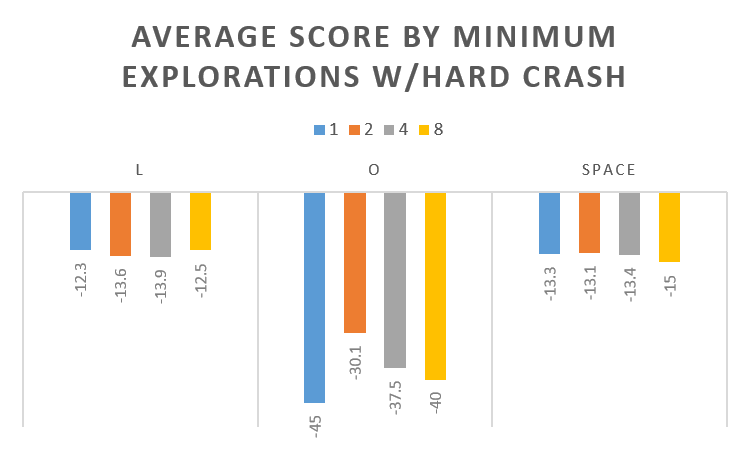
\includegraphics[width=1\textwidth]{img/hard_AvgScore}
    \end{subfigure}
    \begin{subfigure}[b]{0.48\textwidth}
        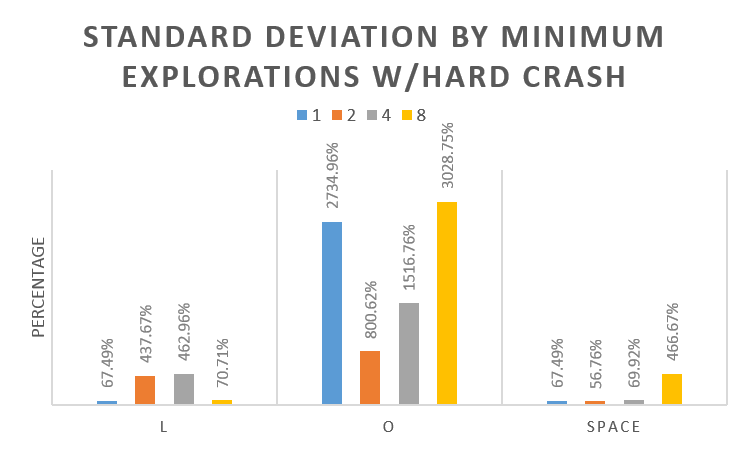
\includegraphics[width=1\textwidth]{img/hard_StDev}
    \end{subfigure}
    \caption{The minimum exploration value for a VI agent was varied between 1, 2, 4, and 8.  Simulation scores were taken across three different maps. Standard deviation analysis measured the variability of scores across the simulations. The results are shown above for each condition under hard crash settings.}
    \label{fig:hardAvgScoreStDev}
\end{figure}

\begin{figure}[h!] 
    \centering
    \begin{subfigure}[b]{0.48\textwidth}
        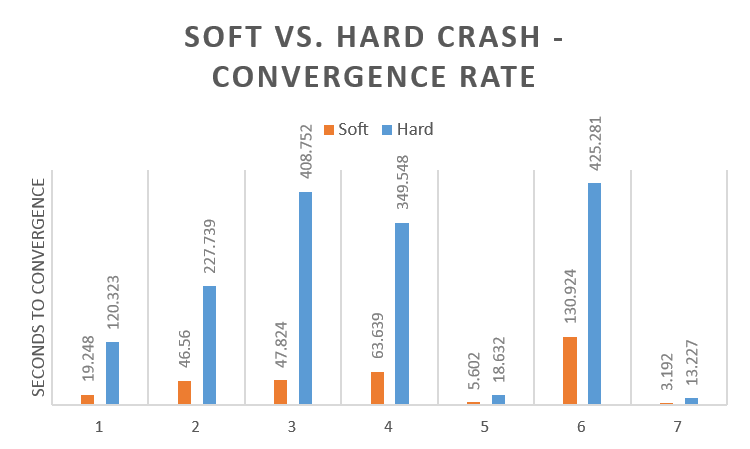
\includegraphics[width=1\textwidth]{img/softVhard/VI/Time}
    \end{subfigure}
    \begin{subfigure}[b]{0.48\textwidth}
        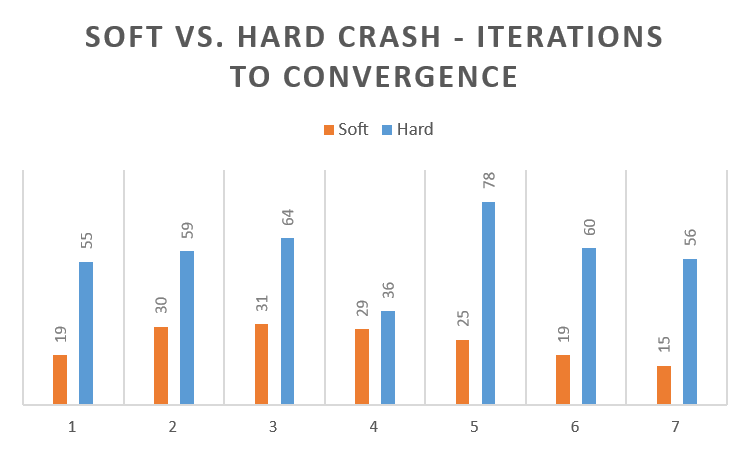
\includegraphics[width=1\textwidth]{img/softVhard/VI/Iter}
    \end{subfigure}
    \caption{The seconds and iterations taken for a Q agent's state-action values to reach an equilibrium state, or convergence, on maps L, O, and Space are shown above. The minimum exploration value was varied between 1, 2, 4, and 8 for both hard and soft crash settings.  The comparison is shown above.}
    \label{fig:svhVITimeIter}
\end{figure}
\clearpage

\begin{figure}[h!] 
    \centering
    \begin{subfigure}[b]{0.48\textwidth}
        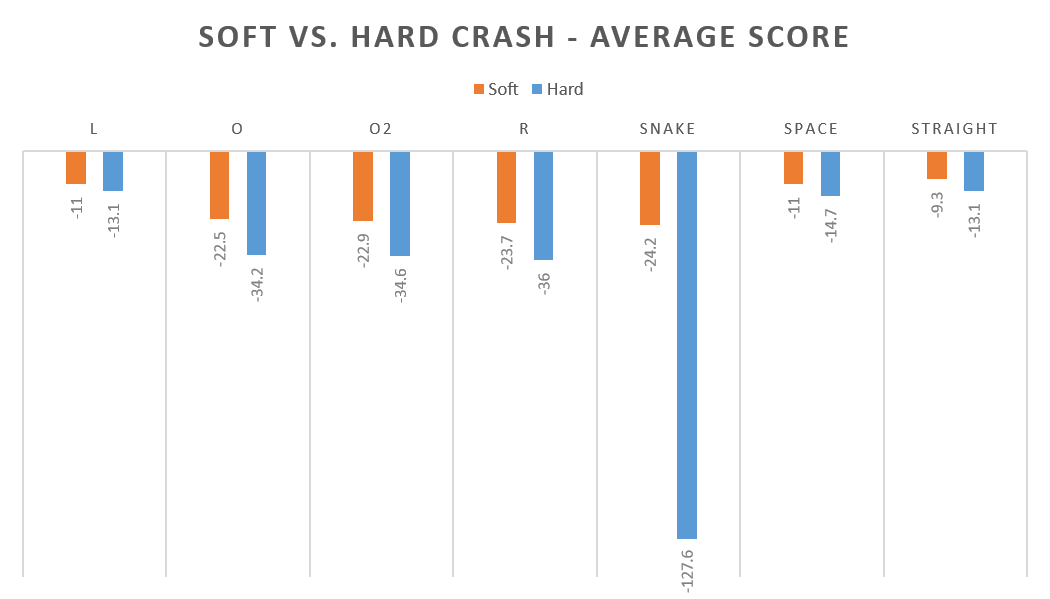
\includegraphics[width=0.9\textwidth]{img/softVhard/VI/AvgScore}
    \end{subfigure}
    \begin{subfigure}[b]{0.48\textwidth}
        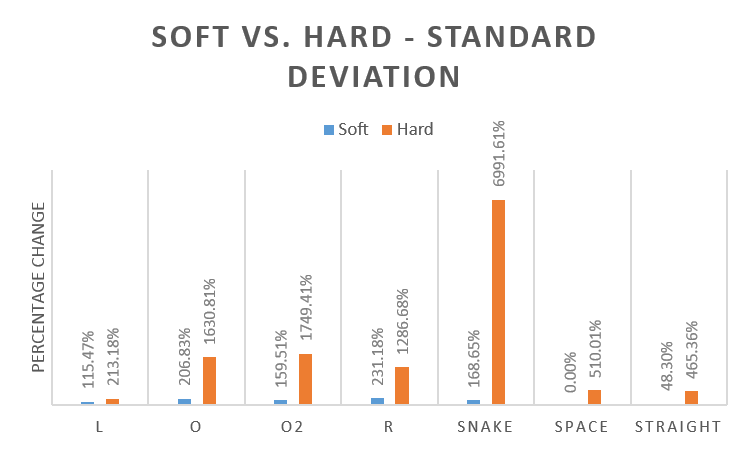
\includegraphics[width=0.9\textwidth]{img/softVhard/VI/StDev}
    \end{subfigure}
    \caption{The minimum exploration value for a Q agent was varied between 1, 2, 4, and 8.  Simulation score averages were taken across three different maps. Standard deviation analysis measured the variability of scores across the simulations. The results are shown above for each condition.}
    \label{fig:svhVIAvgScoreStDev}
\end{figure}
\vspace{-.25em}

\titleline{Experiment 2}
Where Experiment 1 compared the effects of minimum exploration values and crash settings on performance, Experiment 2 focused on the comparative, and perhaps additive, influence of the $\alpha$ learning functions and the discount factor, $\gamma$.  Using the same basic process as in Experiment 1, a Q learner's performance was measured before and after convergence.  The three alpha learning functions, (\ref{eq:alphaN}), (\ref{eq:alpha10N}), and (\ref{eq:alphaNN}), were tested and are compared below.  A polynomial equation of $n$ to the third power was also tested, but is not shown as part of the experiment. While it continued the trend demonstrated in the provided results, it was not significantly different enough from \Fref{eq:alphaNN} to warrant further testing.

% ALPHA:
\begin{figure}[h!] 
\renewcommand\thesubfigure{\roman{subfigure}}
    \centering
    \begin{subfigure}[b]{0.48\textwidth}
        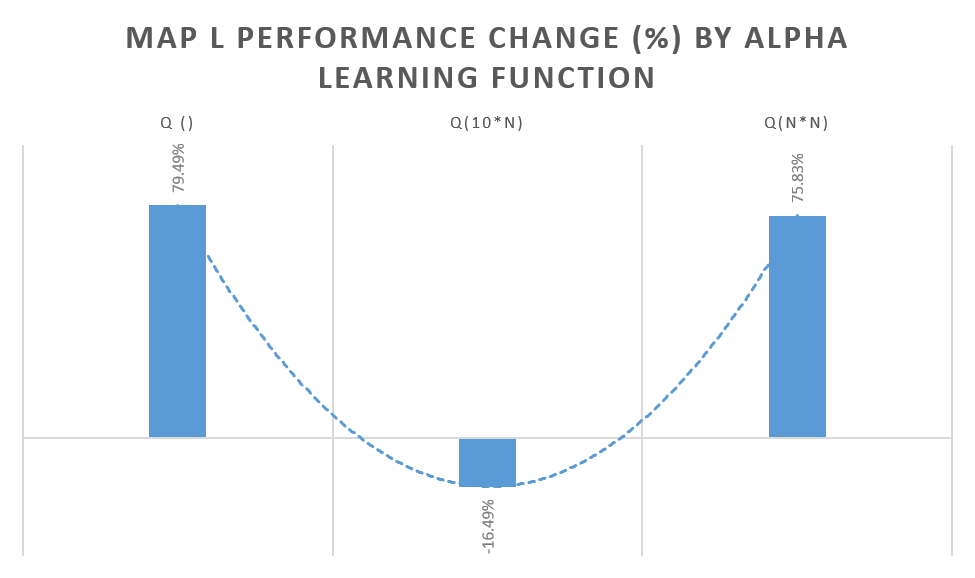
\includegraphics[width=1\textwidth]{img/L_Alpha/AvgScore}
        \caption{Average score}
    \end{subfigure}
    \begin{subfigure}[b]{0.48\textwidth}
        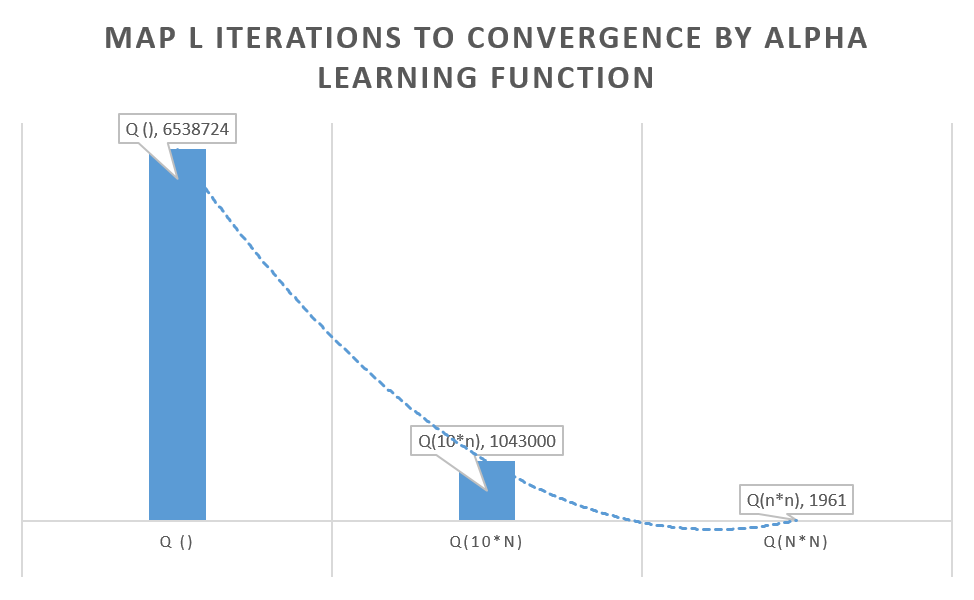
\includegraphics[width=1\textwidth]{img/L_Alpha/Iter}
        \caption{Iterations}
    \end{subfigure}
    \\
    \begin{subfigure}[b]{0.48\textwidth}
        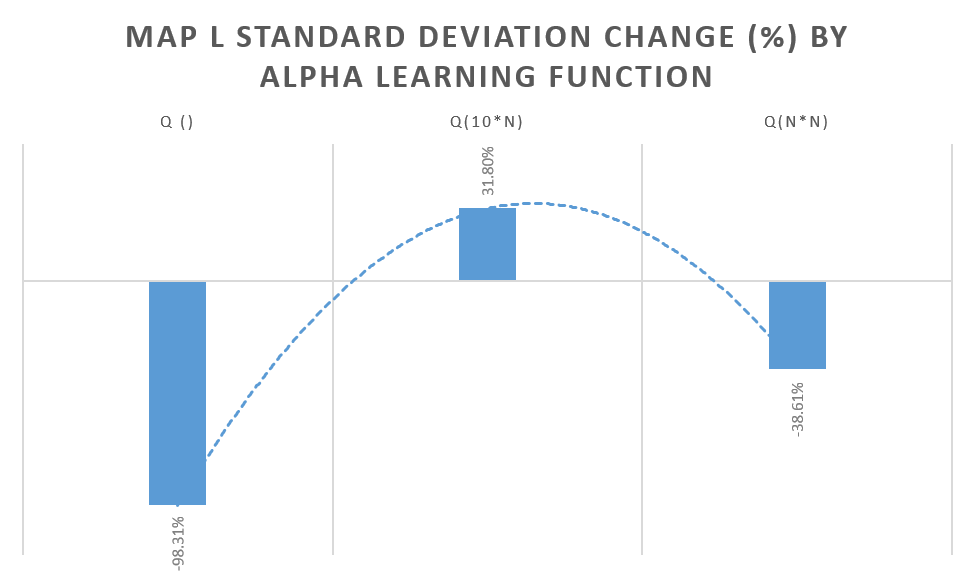
\includegraphics[width=1\textwidth]{img/L_Alpha/StDev}
        \caption{Standard deviation}
    \end{subfigure}
    \begin{subfigure}[b]{0.48\textwidth}
        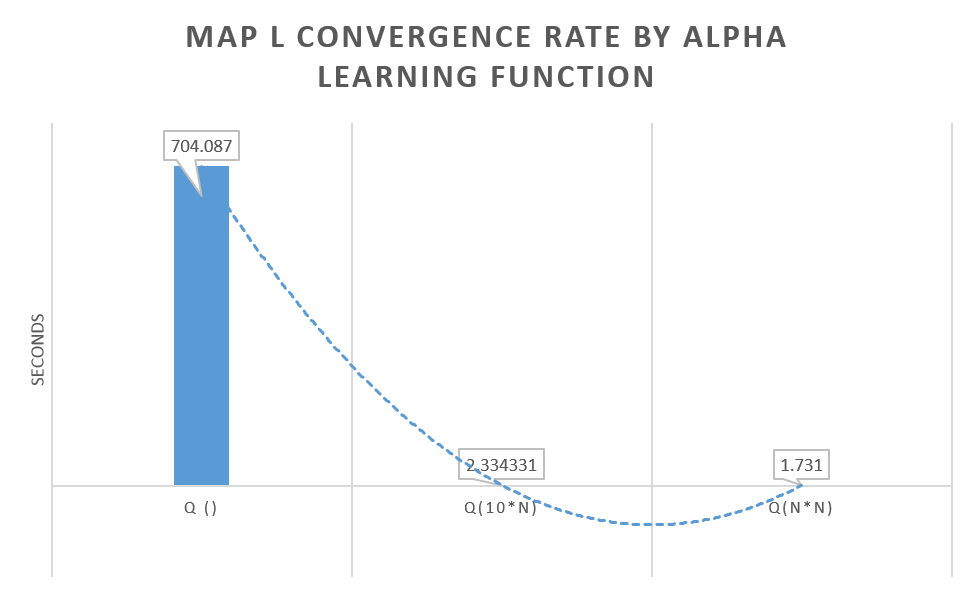
\includegraphics[width=1\textwidth]{img/L_Alpha/Time}
        \caption{Time}
    \end{subfigure}
    \caption{Average score improvement, iterations and time to convergence, and standard deviation change are shown for varying alpha learning function formulae running on L-track.}
    \label{fig:lalphaTimeIterAvgScoreStDev}
\end{figure}
\clearpage

\begin{wrapfigure}{r}{0.8\textwidth} 
  \centering
  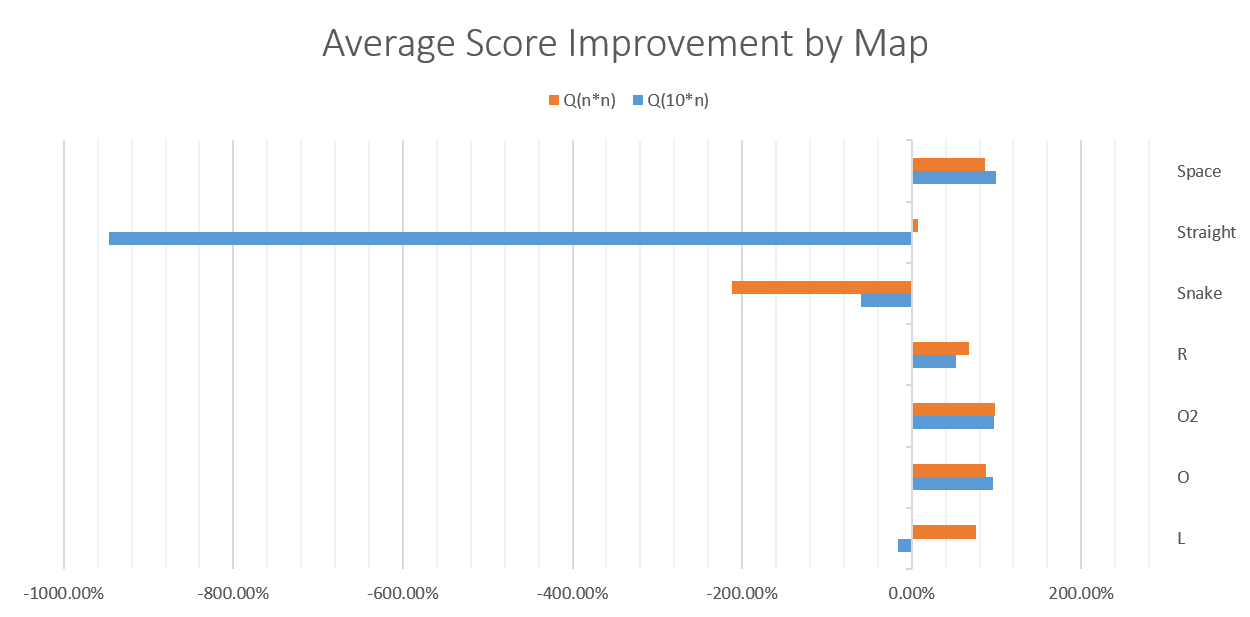
\includegraphics[width=.76\textwidth]{img/avgScore_Maps}
  \caption{The change in average scores of alpha learning functions \Fref{eq:alpha10N} and \Fref{eq:alphaNN} are compared here across all seven maps.}
  \label{fig:mapsAvgScore}
\end{wrapfigure}

Only L-track is used in the comparison, as the data collection process with an alpha learning function independent of the number of state-action visit events, $n$, such as (\ref{eq:alphaN}), might take nearly a day's worth of iterations to converge.  Unlike other maps, which didn't show convergence progress even after 7+ hours of iterations, L-track was exceptionally fast, taking a mere 11.7 minutes.  The remaining maps compared only alpha learning functions (\ref{eq:alpha10N}) and (\ref{eq:alphaNN}), as presented in Figure \ref{fig:mapsAvgScore}.

% GAMMA:
\begin{figure}[h!] 
\renewcommand\thesubfigure{\roman{subfigure}}
    \centering
    \begin{subfigure}[b]{0.49\textwidth}
        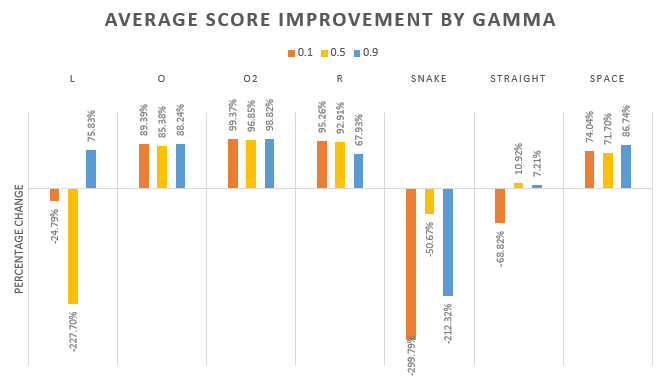
\includegraphics[width=1\textwidth]{img/gamma/AvgScore}
        \caption{Average score}
    \end{subfigure}
    \begin{subfigure}[b]{0.49\textwidth}
        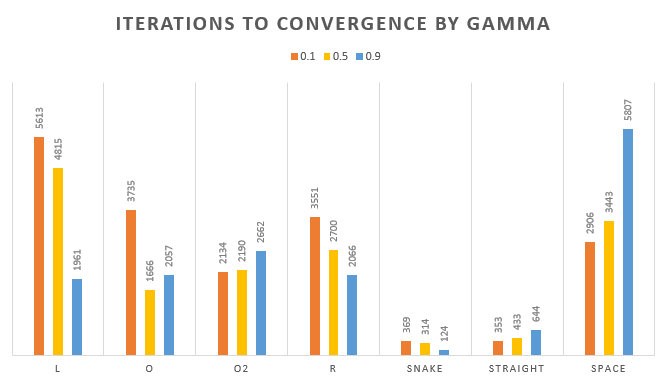
\includegraphics[width=1\textwidth]{img/gamma/Iter}
        \caption{Iterations}
    \end{subfigure}
    \\
    \begin{subfigure}[b]{0.49\textwidth}
        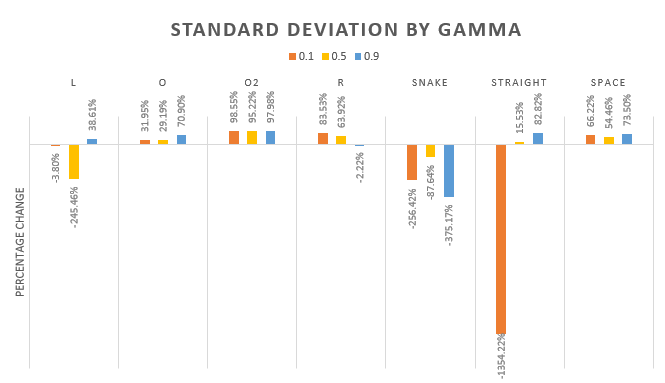
\includegraphics[width=1\textwidth]{img/gamma/StDev}
        \caption{Standard deviation}
    \end{subfigure}
    \begin{subfigure}[b]{0.49\textwidth}
        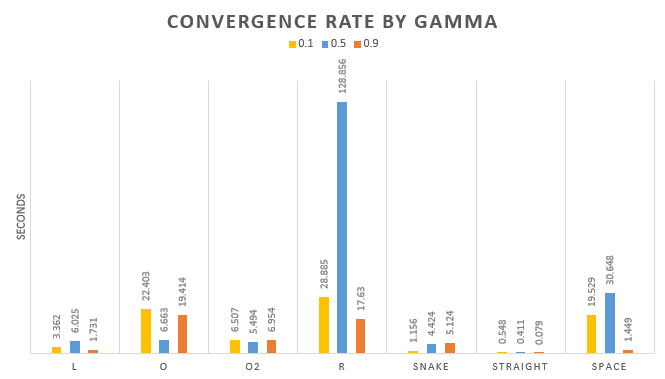
\includegraphics[width=1\textwidth]{img/gamma/Time}
        \caption{Time}
    \end{subfigure}
    \caption{Average score improvement, iterations and time to convergence, and standard deviation change are shown for gamma factors 0.1, 0.5, and 0.9.}
    \label{fig:gammaTimeIterAvgScoreStDev}
\end{figure}
\vspace{-1em}

The discount factor, $\gamma$, on the other hand, did not produce any such difficulties. Data was collected across all seven tracks in the same manner, recording performance before and after convergence, as well as the time and iterations taken to reach convergence.  Since the gamma factor is generally a decimal number between 0 and 1, the gamma factors compared were 0.1, 0.5, and 0.9.

% -------------------------------- DISCUSSION:
\clearpage
\section{Discussion}

\titleline{Experiment 1}

\begin{wrapfigure}{r}{0.65\textwidth} 
    \centering
  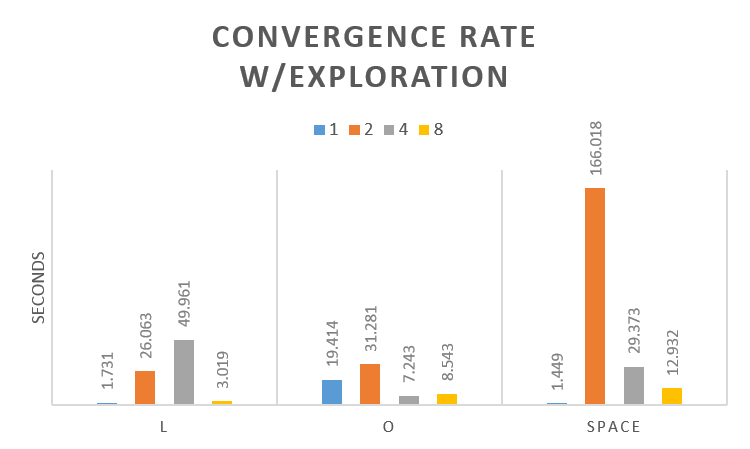
\includegraphics[width=.7\textwidth]{img/minE/Time}
  \caption{By map, the time in seconds for a Q learner to converge on an optimal policy under $N_e$ values of 1, 2, 4, and 8 is shown.}
  \label{fig:minETime}
\end{wrapfigure}

Across all maps, there appears to be a clear Bell Curve for convergence rates.  While processing time peaks with a minimum exploration value, $N_e$, of 2, the process returns to a more rapid convergence again as $N_e$ increases to 8. In the case of O-track, the convergence was even \emph{more} efficient at 4 and 8, than it was when $N_e$ equalled 1. Perhaps this bolstered performance suggests an inherent trade-off at work in the exploratory agent.  A more inquisitive learner takes greater risks, and is more likely to branch out and explore new territory.  Contrarily, on a large map or in an environment with wide open space, this same penchant for exploration may cost the agent valuable time wandering in unproductive search patterns.  This would explain the severe penalty to convergence rate seen in Space-track at 2 $N_e$, where much of the surrounding terrain is extraneous.

\begin{wrapfigure}{l}{0.65\textwidth} 
    \centering
  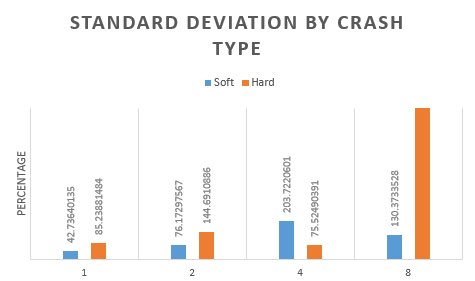
\includegraphics[width=.6\textwidth]{img/softVhard/Q/StDevFlat}
  \caption{Average standard deviation is computed from a series of 10 Q learner trials on L-track, under both soft and hard crash conditions.}
  \label{fig:svhQStDevFlat}
\end{wrapfigure}

More interesting than this sudden increase, however, is its rapid decrease once more on the "right side" of the Bell Curve.  The speed of convergence seems to overcome the main "hump" of the Bell Curve at 4, in the case of L-track, and at 2 on the O and Space tracks.  Referring back to \Fref{fig:permutations}, we see that O-track is approximately $38\%$ larger than L-track, and Space track is over 5 times as large.  This suggests a possible explanation for the apparent shifts in the optimal exploration limit, and perhaps shed light on the paradox of artificial inquisitiveness in itself.

As the minimum exploration limit grows larger it, indeed, encourages the agent to explore, but it likewise prevents the agent from earlier distinguishing between the explored and unexplored.  It effectively delays the Q learner's judgment on whether or not a state-action has been adequately investigated, leaving the agent just as likely to dally in locations it has already found useless several times, as it is to spread out and discover new portions of the map.  By this logic, the Bell Curve might be describing a weakness in the nature of inquisitiveness itself - if one becomes so inquisitive as to spend inordinate amounts of time on local phenomena, one essentially begins to behave as if they are not adventurous or inquisitive at all.

The behavior observed when we increase the possible penalty for exploration is telling.  At higher values of $N_e$, standard deviation is consistently lowered in order to achieve an optimal policy, regardless of the risk involved.  It appears that the inquisitiveness detracts from the optimal policy's variability, rather than adds to it.  Applying our earlier assumption on inquisitiveness, a feasible explanation is that as Q learners are encouraged to explore their local area more deeply, the resulting values become more severely discouraging.  This would essentially "hedge" the path to the goal, creating more powerful deterrents to any direction other than directly towards the finish.  In \Fref{fig:svhQAvgScoreStDev}, we see this evidenced by the remarkably stable score improvement across higher values of $N_e$, but significant performance improvement from soft to hard, when $N_e$ equals 1.  Similarly in \Fref{fig:svhQTimeIter}, we see a distinct decrease in iterations and seconds til convergence, after it crosses the threshold of 2 or 4, respectively.  State-actions values are set very clearly to instruct the agent towards one distinct plan, in a manner much like a biological organism acquiring a very strong response to a harmful stimulus, such as avoiding a lethal predator.

\begin{wrapfigure}{l}{0.65\textwidth} 
    \centering
    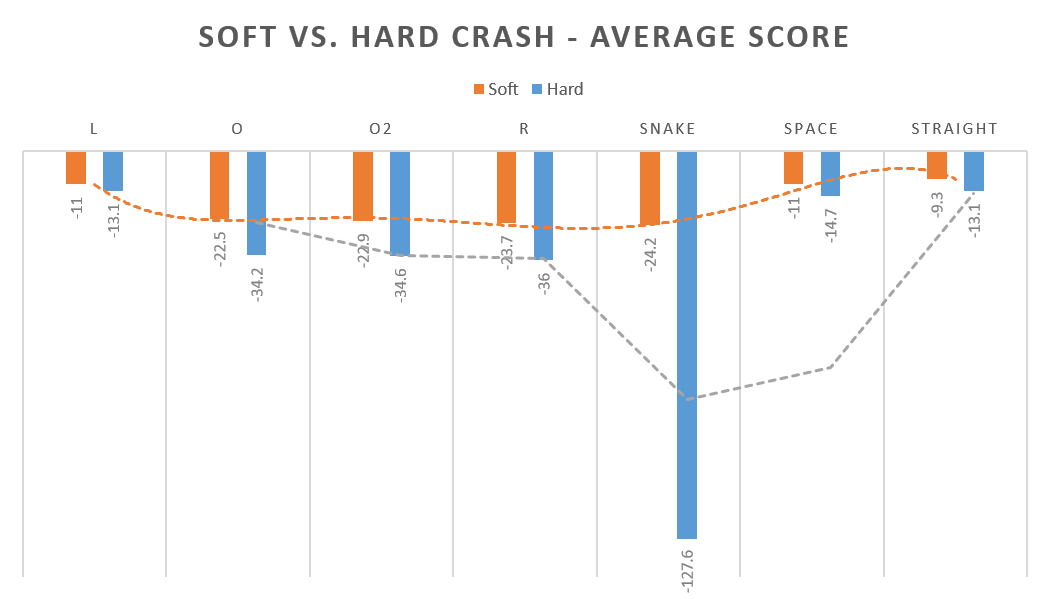
\includegraphics[width=.6\textwidth]{img/softVhard/VI/AvgScoreWLines}
    \caption{The dotted lines on this figure are only present to highlight the distinct negative growth of the score from soft to hard crash setting on each map.}
    \label{fig:svhVIAvgScoreWLines}
\end{wrapfigure}

The VI agent demonstrates the same principles of behavior, when altering both the crash condition and $N_e$.  While strictly comparing soft versus hard crash average scores, we see in \Fref{fig:hardvVq} that the VI agent performs consistently worse, when a hard crash penalty is introduced, and drastically worse on O-track.  The trend seems to indicate that the VI agent has a more difficult time instituting strict protocols to adapt to the hard crash environment.  Perhaps by working backwards, the "trickle down" effect implemented by the VI has trouble creating a harsher values gradient to control for environmental contingencies.  Since each action has a $10\%$ probability of failing, the stochastically weighted VI utility function, \Fref{eq:utility}, may miss valuable chances to optimize its policy by growing overly cautious in its value estimates.

Indeed, the VI agent appears to be less affected by changes to $N_e$.  In \Fref{fig:minETimeIter}, we see a perfect plateau as all VI agents converge after the same number of iterations, regardless of the value of $N_e$.  Likewise, in \Fref{fig:minEAvgScoreStDev}, there is relatively little change in performance, save a decreased average score with increasing $N_e$ values on the O-track.  Perhaps O-track, with its relatively narrow turns exacerbates the VI agents difficulty with forming a sufficiently "padded" value gradient.  Nonetheless, while the VI learner's convergence rate remains relatively unaffected, the major point of change is in the standard deviation. \Fref{fig:minEAvgScoreStDev} shows radical changes in VI as the inquisitiveness of the learner increases, especially when it is to its detriment, as in O-track.  While L-track demonstrates yet another Bell Curve, O-track shows an upside-down Bell Curve of sorts.  We know the VI agent performs poorly on O-track, and this is reflected again in its average scores.  As the standard deviation drops, the average score rises.

\begin{wrapfigure}{l}{0.65\textwidth} 
    \centering
    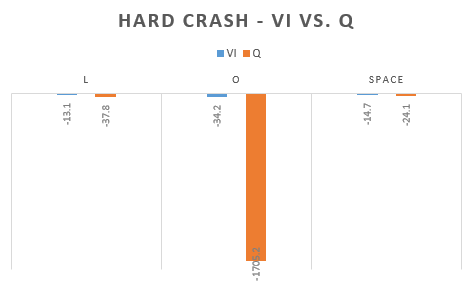
\includegraphics[width=.6\textwidth]{img/hard_vVq}
    \caption{A comparison of the average scores of a VI and Q agent taken over 10 trials on three different maps under hard crash conditions, at $N_e =1$.}
    \label{fig:hardvVq}
\end{wrapfigure}

Interestingly enough, we see the converse here of the phenomenon displayed in Q.  For both the highest and lowest value of $N_e$ performance is lower, but with values of 2 or 4, the performance cost is relatively less.  Returning to our earlier assumption, if inquisitiveness truly lies on a Bell Curve, then perhaps the adventurous tendencies peaking at $N_e$ values 2 and 4 are beneficial in this circumstance, partially offsetting the hard crash penalty.  Perhaps a VI agent with a greater inquisitive "instinct" will persist in following the proper value gradient longer, while simultaneously balancing not becoming \emph{too} side-tracked, as to veer off-course.  In other words, the VI agent a visitation event limit at 2 or 4 might strike a better balance between charging off-course, and myopically exploring everything within the local area.
\\ \\

\titleline{Experiment 2}

Dealing exclusively with the Q-learning agent in Experiment 2, we varied the exponential power of its alpha learning function.  Between \Fref{eq:alphaN}, \Fref{eq:alpha10N}, and \Fref{eq:alphaNN}, we see a definite increase in learning convergence rate, as expected.  Interesting and unexpected, however, is that the \emph{performance} does not necessarily increase.

\begin{wrapfigure}{r}{0.7\textwidth} 
  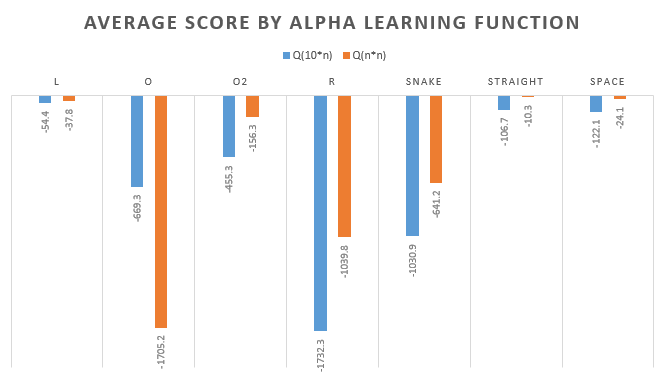
\includegraphics[width=0.67\textwidth]{img/alpha_AvgScore}
  \caption{The average scores of the two alpha learning functions \Fref{eq:alpha10N} and \Fref{eq:alphaNN} are compared over all seven test tracks.}
  \label{fig:mapsAvgScoreMaps}
  \vspace{-.5em}
\end{wrapfigure}

In \Fref{fig:lalphaTimeIterAvgScoreStDev}, we see that an alpha learning factor constant, \Fref{eq:alphaN}, and an alpha learning function of $n$ to the second power yield comparable average scores, while the performance of \Fref{eq:alpha10N}, $n$ to the first power, suffers.  These results, however, regard Q agent performance on just the L-track map.  Viewing \Fref{fig:mapsAvgScore}, we observe varied levels of performance \emph{improvement} across all maps.  Strangely, it appears that $n^1$ performs better, or at least not as badly as $n^2$, on more complex maps, such as Snake-track or R-track, while performing relatively badly on simple tracks, such as Straight-track.  Since an alpha learning function dividing $\alpha$ by $n^2$ rapidly diminishes update weight once $n$ is greater than one, or the particular state-action has been visited more than once, a Q agent operating under \Fref{eq:alphaNN} might learn so rapidly, with minimal revisions or updates, that it somewhat neglects the value refinement process within each iteration.  By doing so, the gradient of state-action values across the map may not be as refined as a $n^1 \alpha$ function, and, thus, has a greater tendency to veer off-course on unforgiving maps, such as Snake-track.

\Fref{fig:lalphaTimeIterAvgScoreStDev} also shows a conversely distributed standard deviation change.  In other words, the more effectively the alpha learning function decreased the variability in its simulation scores, settling on an optimal policy, the more its average score improved.  By the definition of convergence, this result is intuitive\cite{textbook}, however, here again the alpha learning function with $n^1$ yields the weakest performance, rather than the fixed constant.  This also shows us that the average score, not only is outperformed, but \emph{decreases} after convergence.

When $n$ is removed from the alpha learning function, regardless of any added constants, it becomes an alpha learning factor.  Thus, the Q learner closely returns to the behavior of a Q-learning agent without an exploration function.  Thus, the results suggest that the benefits of employing a learning function are more noticeable at higher powers of $n$.  Additionally, if a Q learner is to be applied to a specific problem, the relative task simplicity or complexity of the problem may indicate an optimal alpha learning equation exists at a particular power of $n$.

As the $\alpha$ learning function decreases the influence of future updates, it limits the effect of future state-actions on its current state.  The discount factor, $\gamma$,  creates a similar "tunnel-vision" effect, with lower values resulting in the devaluation of state-action values relating to position further away, or in the "future".  By directing the value that an agent places on future rewards versus rewards in the present, the discount factor effectively controls the agent's "greed"\cite{textbook} and its perception of the value of time.  If a reward several iterations in the future outweighs the cost to obtain it, the reward may become as valuable as an immediate reward.

\Fref{fig:gammaTimeIterAvgScoreStDev} demonstrates how interactions between $\gamma$ and $\alpha$ learning functions can have a host of curious effects.  L-track performance suffers greatly with lower levels of gamma, suggesting that more "short-sighted" behavior lowers performance.  However, the damage is greatest when $\gamma$ equals 0.5.  Perhaps, in this instance a higher score is best obtained by committing to one strategy, rather than "straddling the fence".  Yet, the converse appears to be true for Snake-track, the midway gamma value yielding the \emph{lowest decrease} in performance.  On complex tracks, such as Snake-track, which require a great deal of task-switching, perhaps it is best to \emph{not} push an agent's policy too far in either direction, as this results in a too-cautious or too-brash Q learner.  This would serve to explain the decreased performance on Straight-track at a $\gamma$ value of 0.1, as well.  On such a simple map, overly-cautious, short-sighted agents would over-compensate in an incredibly straight-forward environment.

These decreases in average scores coincide with decreases in standard deviation as well.  The more varied the outcomes a Q learner's policy produces, the lower its average score.  Surprisingly, these decreases do not always correspond to faster convergence rates.  L-track and R-track, for example, both have relatively high (or slow) convergence rates, spending plenty of time and iterations working towards convergence.  Thus, the problem does not seem to be dependent on the \emph{rate} at which the Q-learning policy converges, or the "passage of time", but on the Q learner's perception of it - the methodology by which the agent handles future state-actions.  Lower $\gamma$ values make the Q agent myopic, and might artificially simulate a disability to plan ahead, or anticipate future movements.  When movements require a persistent movement action towards an end goal, such as in Straight-track, this inability to "see" the finish line significantly hurts performance.

% -------------------------------- CONCLUSIONS:
\section{Conclusions}
    Reinforcement learning is a complex, dynamic process involving the interplay of a myriad of motivating, and demotivating, factors, which provide a learner with their unique perception and understanding of the environment.  In Artificial Intelligence, these factors take the form of stochastic variables, participating in mathematical models that simulate the seemingly simple process of learning.

    Inquisitiveness is an important player in the modeling process, as one might intuitively expect.  Exploration functions help to model and balance the trade-offs between the risks and rewards of adventurous behavior.  However, sometimes mathematical models model unexpected qualities as well.  The minimum exploration limit, $N_e$, controls the number of visits an agent make to a particular state-action before that state-actions reward is diminished from the optimistic promise of an unexplored state.  This value, however, yields behavior consistent with a lower minimum exploration limit, 1, once it crosses a certain threshold (2 or 4 in the experiments described in this paper).  A virtual Bell Curve, data results suggest that the more "inquisitive" an agent becomes, or the more visit events must occur before it marks a state-action as sufficiently explored, the more effort it appears to expend fixating on its local environment.
    
    Two more important players, the $\alpha$ learning function and the discount factor $\gamma$, model a reinforcement learning agent's perception of time and distance, an essential part of any learning.  Risk and reward evaluation both depend on an agent's ability to distinguish worthwhile pursuits.  Motivation itself lies in the probabilistic comparisons of costs and yields.  The $\alpha$ learning factor manipulates the rate at which a Q-learning agent converges on an optimal policy of action, but it also affects the agent's attitude towards future experiences.  A polynomial function, an exploratory $\alpha$ learning function shows varying performance and convergence rate as the exponential power of $n$ varies.  An $\alpha$ learning function, rather than $\alpha$ \emph{factor}, may allow an agent to better discriminate when update information is still valuable.  However, \Fref{eq:alpha10N} with $n^1$ appears to perform better under conditions involving complex environments with frequent task-switching, while \Fref{eq:alphaNN} with $n^2$ appears to perform better under conditions involving simpler environments or in task require greater persistence and less task-switching.  Together the alpha learning function and discount factor produce a unique temporospatial perspective that helps orient a Q-learning agent to its environment.


\clearpage
\section{Appendix}

\listoffigures

\appendix
\section{Q-learning: Alpha}
\raisebox{0cm}{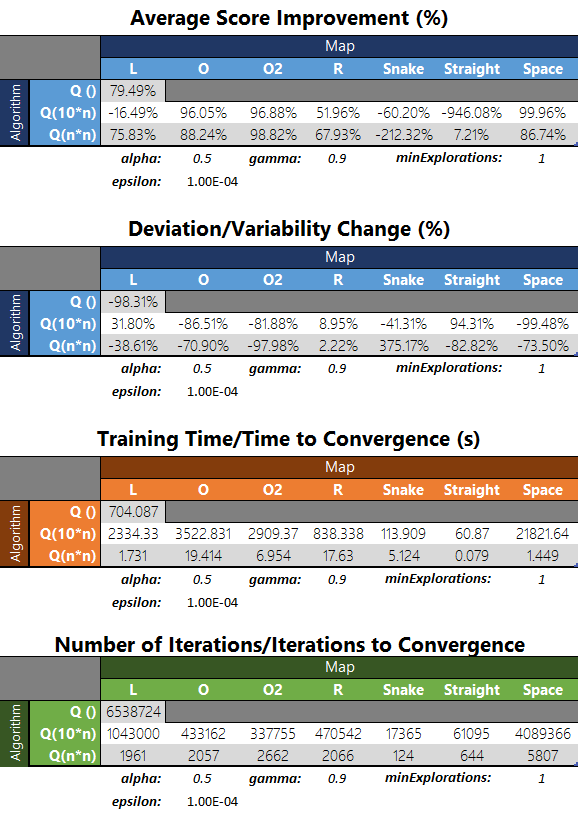
\includegraphics{img/appendix/q_alpha_info_charts}} \newpage
\raisebox{0cm}{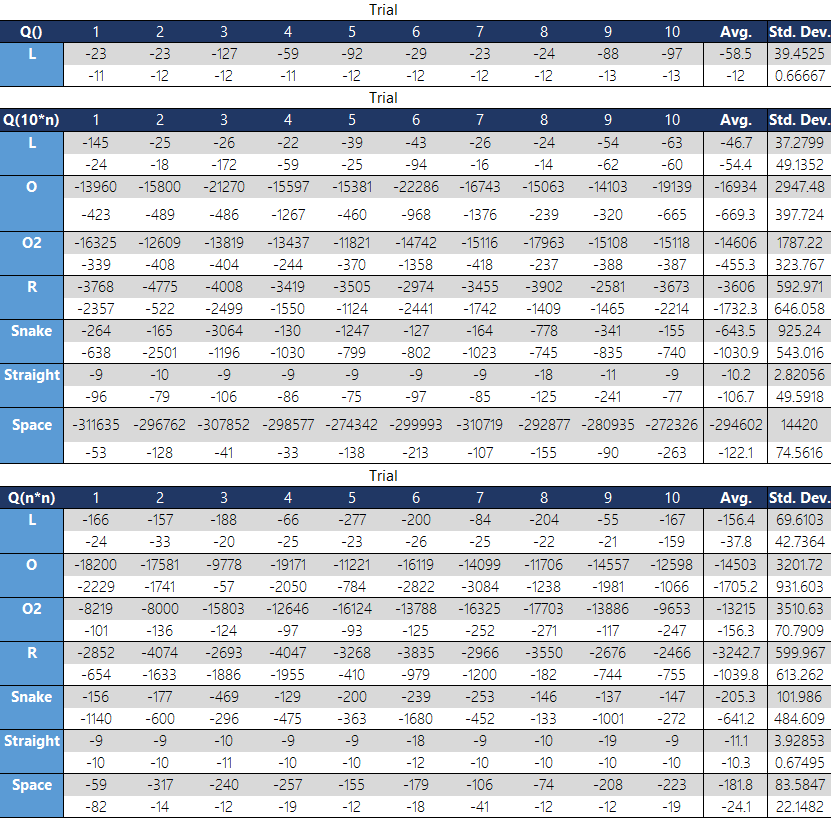
\includegraphics[width=16cm]{img/appendix/q_alpha_trials}}

\section{Q-learning: Gamma}
\raisebox{0cm}{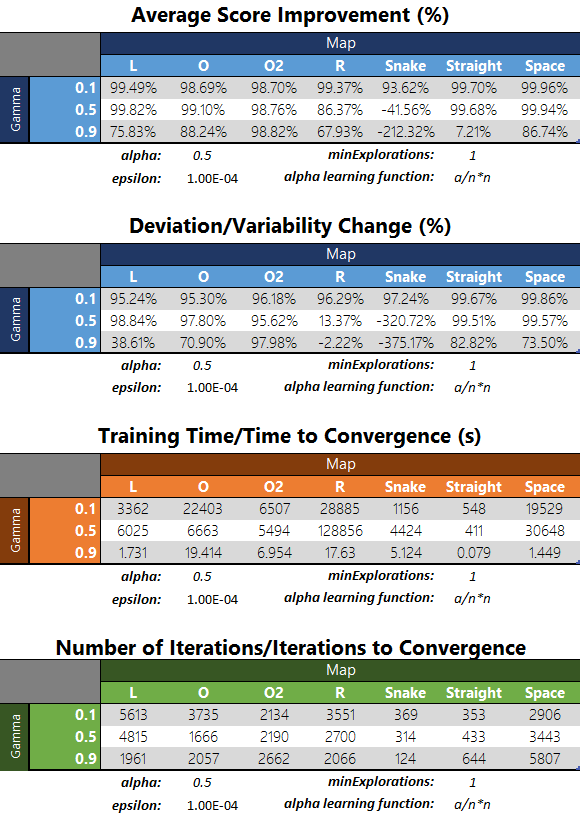
\includegraphics{img/appendix/q_gamma_info_charts}} \newpage
\raisebox{0cm}{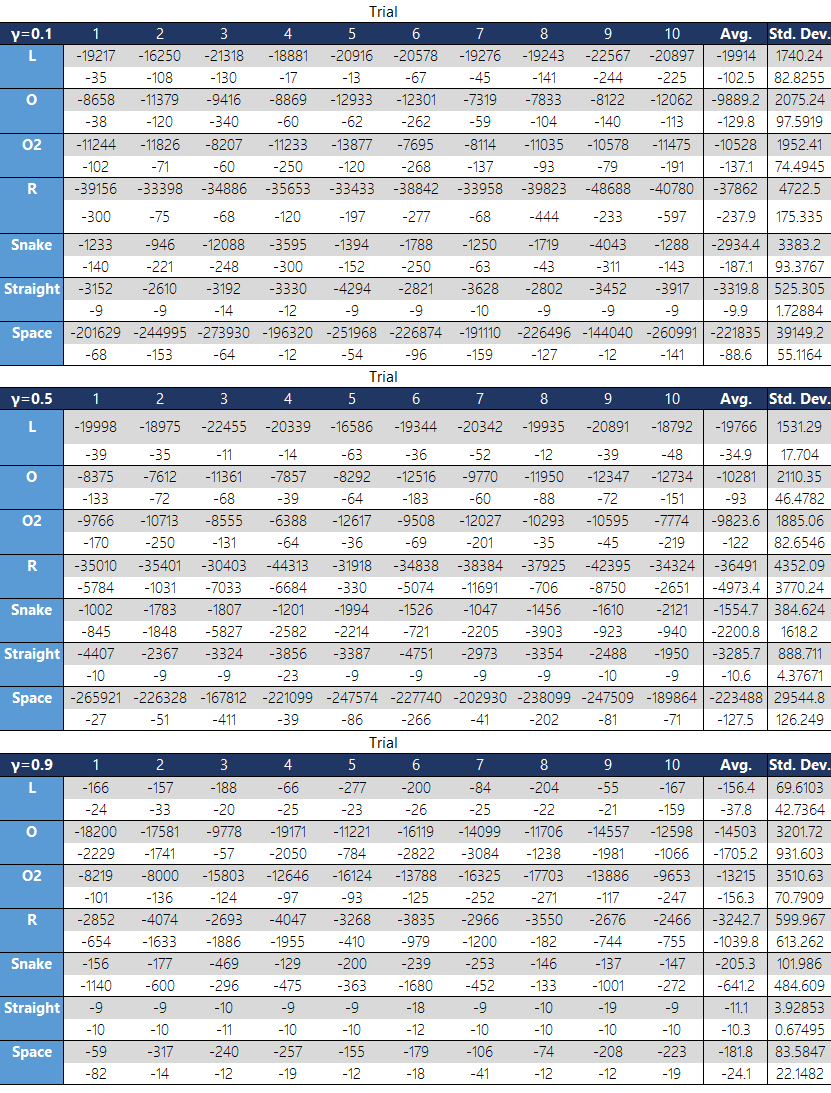
\includegraphics[width=16cm]{img/appendix/q_gamma_trials}}

\section{Q-learning: Minimum Exploration}
\raisebox{0cm}{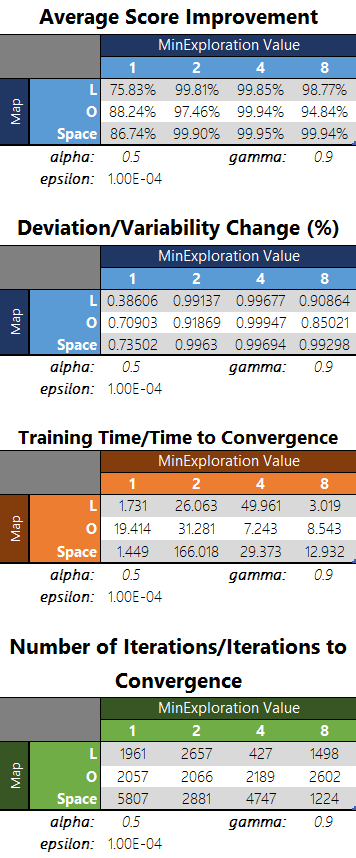
\includegraphics{img/appendix/q_min_exp_info_charts}} \newpage
\raisebox{0cm}{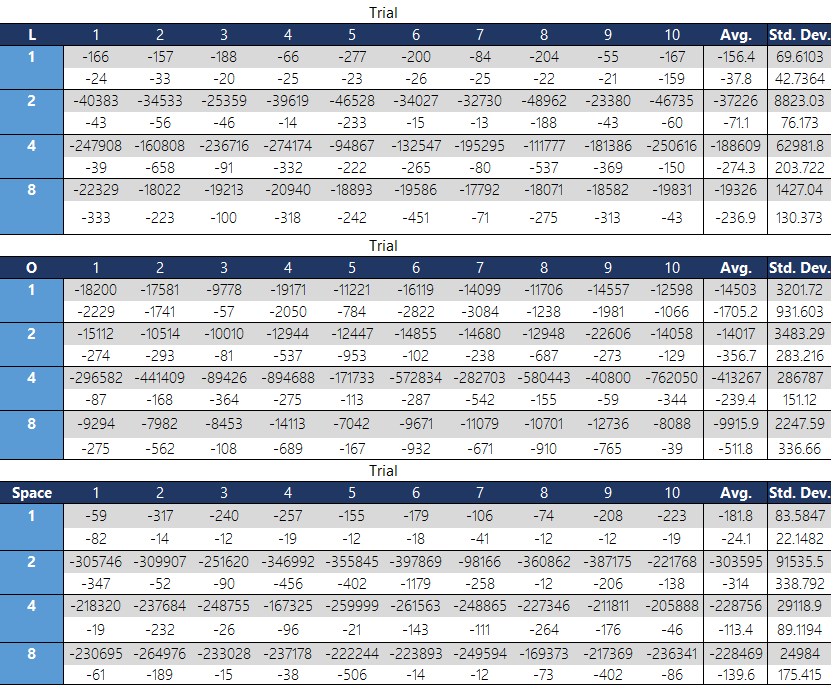
\includegraphics[width=16cm]{img/appendix/q_min_exp_trials}}

\section{Value Iteration learning: Hard Crash}
\raisebox{0cm}{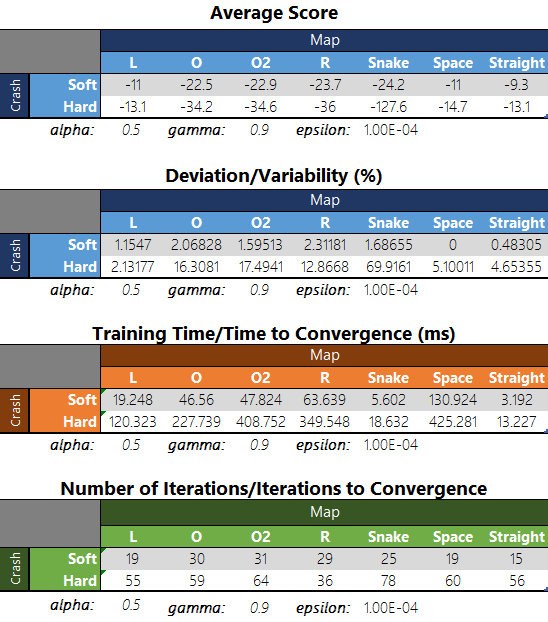
\includegraphics{img/appendix/vi_hard_crash_info_charts}} \newpage
\raisebox{0cm}{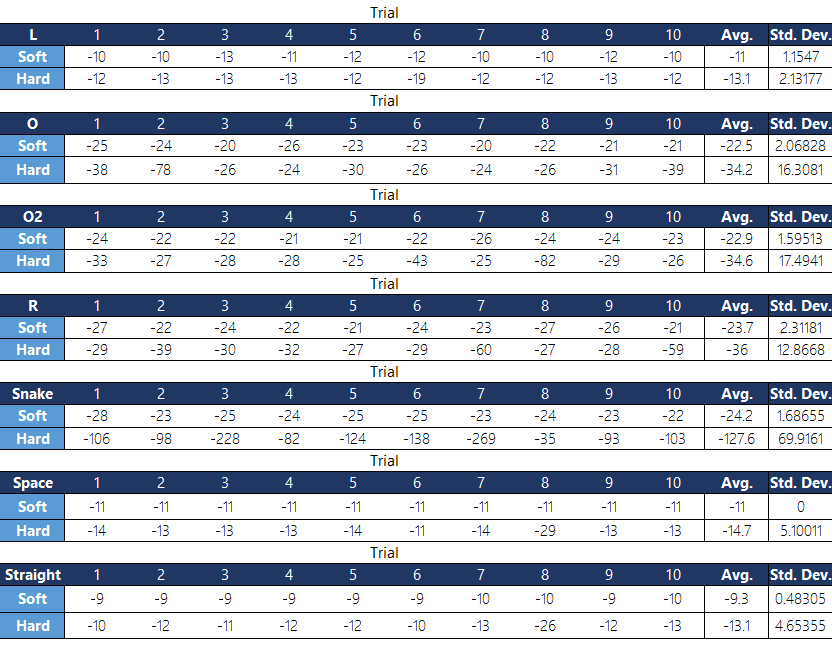
\includegraphics[width=16cm]{img/appendix/vi_hard_crash_trials}}

\begin{thebibliography}{1}
\bibitem{textbook} Russell, Stuart J., Peter Norvig, and Ernest Davis. {\em Artificial Intelligence: A Modern Approach.}  Upper Saddle River, NJ: Prentice Hall, 2010.
\bibitem{classnotes} Mitchell, Ben. {\em CS 335/435 - Artificial Intelligence.} 2015.
\bibitem{final} Mitchell, Ben. "Final Project (Homework 5): Reinforcement Learning." (n.d.): n. pag. CS335/435 - Artificial Intelligence. Benjamin Mitchell, 11 Apr. 2015. Web. 8 May 2015.
\bibitem{cogsci} Gazzaniga, Michael S., Richard B. Ivry, and G. R. Mangun. {\em Cognitive Neuroscience: The Biology of the Mind.} New York: W.W. Norton, 2014. Print.
\end{thebibliography}

\end{document}